\parindent=0em
\subsection{Videojuegos}
\noindent

El impacto de la realidad mixta tampoco podía quedar de lado dentro del mundo de los videojuegos como es natural. Pese al gran potencial que esta tecnología presenta para la industria del videojuego, es un terreno todavía muy poco explorado en comparación a los videojuegos en AR. En realidad aumentada existen videojuegos de éxito como \textit{Pokémon GO} o el juego basado en AR con marcadores \textit{Invizimals}. Por ello no se encuentra gran abundancia de videojuegos que exploren este aspecto. Los que a día de hoy existen están únicamente pensados para dispositivos móviles (Android e iOS) y basados en ubicación por GPS. No suelen ser videojuegos cerrados sino más bien prototipos o pruebas de concepto con escasa funcionalidad. \\

Se pueden destacar los siguientes títulos dentro de este ámbito:

\begin{itemize}

\item \textbf{SpecTrek:} El objetivo principal de este videojuego (figura~\ref{fig:SpecTrk}) es que el usuario realice actividad física. Para ello, plantea una serie de lugares que visitar en los cuales existen una serie de enemigos que habrá que derrotar. Cuenta con tres modos de juego distintos, según el tiempo que el usuario quiera estar realizando actividad física. El videojuego utiliza la ubicación GPS del jugador a medida que este se mueve en la realidad para medir la distancia hacia estos enemigos, y una vez se encuentre delante de uno de ellos, tendrá que encontrarlo con la cámara del dispositivo móvil para eliminarlo.

\item \textbf{Ingress:} Dentro de este videojuego, el objetivo será moverse a través del mundo real para conocer distintas obras de arte urbanas así como monumentos o lugares de interés dentro de una ciudad. Para ello, el videojuego sitúa dentro del mundo una serie de portales virtuales que podremos visitar. Es considerado videojuego ya que mientras más lugares de interés se visiten, más aumentará el nivel del jugador. También dispone de una serie de ``minijuegos'' a realizar por el jugador y facilitar la subida de nivel de este.

\item \textbf{Gbanga Zooh:} Gbanga está definido como una experiencia de ``Gaming social''. En este, las tres actividades a realizar son explorar el entorno, recolectar objetos y recursos del mismo y finalmente intercambiarlos con otros jugadores que hayan seguido el mismo proceso. 

\item \textbf{Can You See Me Now?:} Este videojuego es una imitación del tradicional juego de persecución en el que un jugador tenía que alcanzar a otro y este último huir de él. En este caso, ambos jugadores se encuentran en una ciudad y disponen de un equipo GPS así como un Walkie-Talkie. El equipo GPS transmite constantemente su posición a un ordenador y el Walkie-Talkie sirve para comunicarse con la persona que se encuentra en este ordenador.
Esta última persona, que no se encuentra en la ciudad (una por jugador o una por equipo), tiene que guiar a los jugadores para que cumplan su objetivo simplemente viendo sus posiciones en el ordenador y comunicándose mediante voz. \\


\begin{figure}[H]
    \centering
    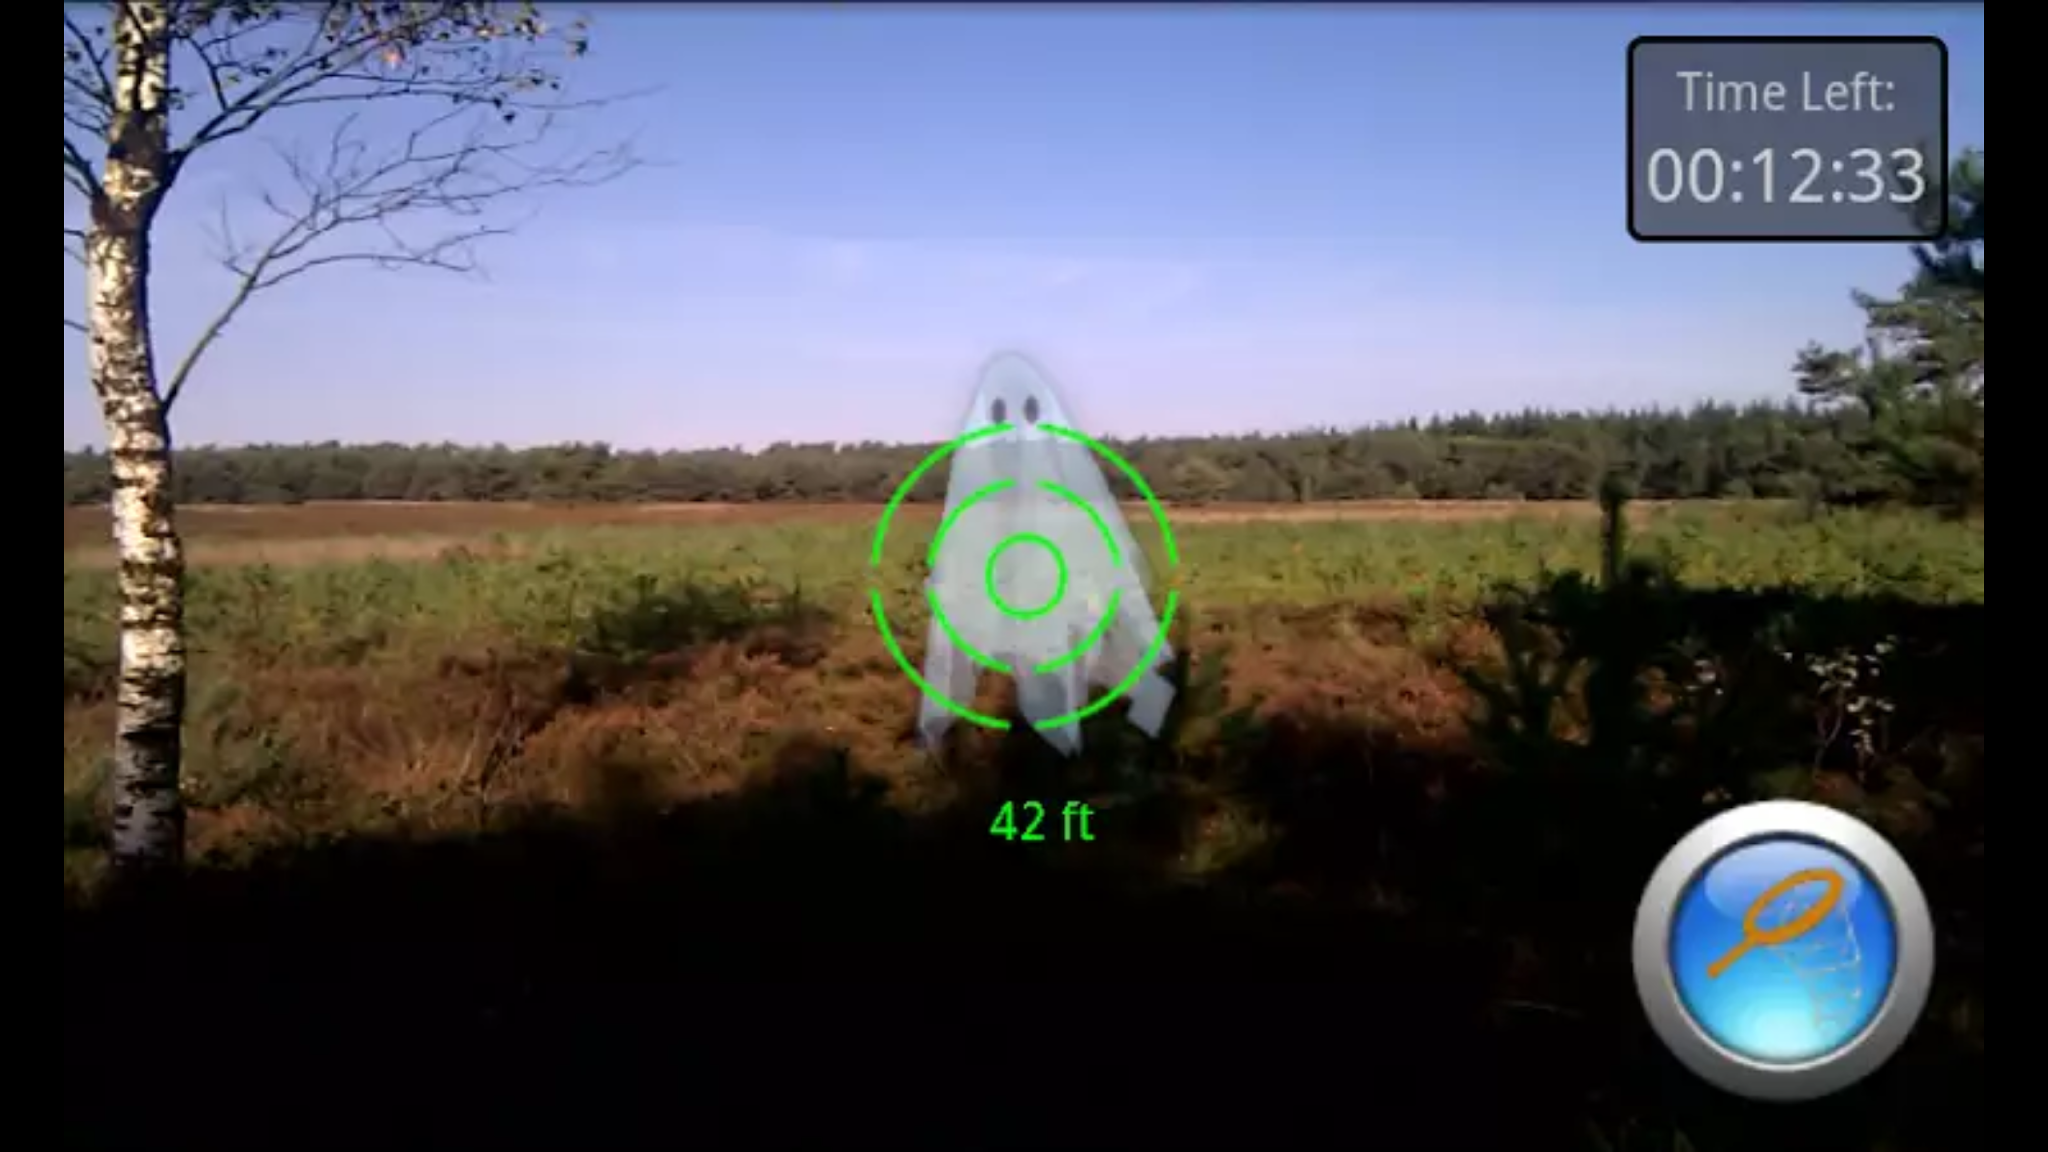
\includegraphics[scale=0.12]{Images/Estado del arte/specktrek.png}
    \caption[Captura de pantalla de \textit{SpecTrek}]{Captura de pantalla de \textit{SpecTrek}\footnotemark.}
    \label{fig:SpecTrk}
\end{figure}

\footnotetext{Fuente: \href{https://play.google.com/store/apps/details?id=com.spectrekking.light&hl=es
}{\nolinkurl{https://play.google.com/store/apps/details?id=com.spectrekking}}}


\end{itemize}